% -*- coding: utf-8 -*-
%-------------------------designed by zcf--------------
\documentclass[UTF8,a4paper,10pt]{ctexart}
\usepackage[left=3.17cm, right=3.17cm, top=2.74cm, bottom=2.74cm]{geometry}
\usepackage{amsmath}
\usepackage{graphicx,subfig}
\usepackage{float}
\usepackage{cite}
\usepackage{caption}
\usepackage{enumerate}
\usepackage{booktabs} %表格
\usepackage{multirow}
\newcommand{\tabincell}[2]{\begin{tabular}{@{}#1@{}}#2\end{tabular}}  %表格强制换行
%-------------------------字体设置--------------
% \usepackage{times} 
\usepackage{ctex}
\setCJKmainfont[ItalicFont=Noto Sans CJK SC Bold, BoldFont=Noto Serif CJK SC Black]{Noto Serif CJK SC}
\newcommand{\yihao}{\fontsize{26pt}{36pt}\selectfont}           % 一号, 1.4 倍行距
\newcommand{\erhao}{\fontsize{22pt}{28pt}\selectfont}          % 二号, 1.25倍行距
\newcommand{\xiaoer}{\fontsize{18pt}{18pt}\selectfont}          % 小二, 单倍行距
\newcommand{\sanhao}{\fontsize{16pt}{24pt}\selectfont}  %三号字
\newcommand{\xiaosan}{\fontsize{15pt}{22pt}\selectfont}        % 小三, 1.5倍行距
\newcommand{\sihao}{\fontsize{14pt}{21pt}\selectfont}            % 四号, 1.5 倍行距
\newcommand{\banxiaosi}{\fontsize{13pt}{19.5pt}\selectfont}    % 半小四, 1.5倍行距
\newcommand{\xiaosi}{\fontsize{12pt}{18pt}\selectfont}            % 小四, 1.5倍行距
\newcommand{\dawuhao}{\fontsize{11pt}{11pt}\selectfont}       % 大五号, 单倍行距
\newcommand{\wuhao}{\fontsize{10.5pt}{15.75pt}\selectfont}    % 五号, 单倍行距
%-------------------------章节名----------------
\usepackage{ctexcap} 
\CTEXsetup[name={,、},number={ \chinese{section}}]{section}
\CTEXsetup[name={(,)},number={\chinese{subsection}}]{subsection}
\CTEXsetup[name={,.},number={\arabic{subsubsection}}]{subsubsection}
%-------------------------页眉页脚--------------
\usepackage{fancyhdr}
\pagestyle{fancy}
\lhead{\kaishu \leftmark}
% \chead{}
\rhead{\kaishu 计算机网络第一次实验}%加粗\bfseries 
\lfoot{}
\cfoot{\thepage}
\rfoot{}
\renewcommand{\headrulewidth}{0.1pt}  
\renewcommand{\footrulewidth}{0pt}%去掉横线
\newcommand{\HRule}{\rule{\linewidth}{0.5mm}}%标题横线
\newcommand{\HRulegrossa}{\rule{\linewidth}{1.2mm}}
%-----------------------伪代码------------------
\usepackage{algorithm}  
\usepackage{algorithmicx}  
\usepackage{algpseudocode}  
\floatname{algorithm}{Algorithm}  
\renewcommand{\algorithmicrequire}{\textbf{Input:}}  
\renewcommand{\algorithmicensure}{\textbf{Output:}} 
\usepackage{lipsum}  
\makeatletter
\newenvironment{breakablealgorithm}
  {% \begin{breakablealgorithm}
  \begin{center}
     \refstepcounter{algorithm}% New algorithm
     \hrule height.8pt depth0pt \kern2pt% \@fs@pre for \@fs@ruled
     \renewcommand{\caption}[2][\relax]{% Make a new \caption
      {\raggedright\textbf{\ALG@name~\thealgorithm} ##2\par}%
      \ifx\relax##1\relax % #1 is \relax
         \addcontentsline{loa}{algorithm}{\protect\numberline{\thealgorithm}##2}%
      \else % #1 is not \relax
         \addcontentsline{loa}{algorithm}{\protect\numberline{\thealgorithm}##1}%
      \fi
      \kern2pt\hrule\kern2pt
     }
  }{% \end{breakablealgorithm}
     \kern2pt\hrule\relax% \@fs@post for \@fs@ruled
  \end{center}
  }
\makeatother
%------------------------代码-------------------
\usepackage{xcolor} 
\usepackage{listings} 
\lstset{ 
breaklines,%自动换行
basicstyle=\small,
escapeinside=``,
keywordstyle=\color{ blue!70} \bfseries,
commentstyle=\color{red!50!green!50!blue!50},% 
stringstyle=\ttfamily,% 
extendedchars=false,% 
linewidth=\textwidth,% 
numbers=left,% 
numberstyle=\tiny \color{blue!50},% 
frame=trbl% 
rulesepcolor= \color{ red!20!green!20!blue!20} 
}
%------------超链接----------
\usepackage[colorlinks,linkcolor=black,anchorcolor=blue]{hyperref}
%------------------------TODO-------------------
\usepackage{enumitem,amssymb}
\newlist{todolist}{itemize}{2}
\setlist[todolist]{label=$\square$}
% for check symbol 
\usepackage{pifont}
\newcommand{\cmark}{\ding{51}}%
\newcommand{\xmark}{\ding{55}}%
\newcommand{\done}{\rlap{$\square$}{\raisebox{2pt}{\large\hspace{1pt}\cmark}}\hspace{-2.5pt}}
\newcommand{\wontfix}{\rlap{$\square$}{\large\hspace{1pt}\xmark}}
%------------------------水印-------------------
\usepackage{tikz}
\usepackage{xcolor}
\usepackage{eso-pic}

\newcommand{\watermark}[3]{\AddToShipoutPictureBG{
\parbox[b][\paperheight]{\paperwidth}{
\vfill%
\centering%
\tikz[remember picture, overlay]%
  \node [rotate = #1, scale = #2] at (current page.center)%
    {\textcolor{gray!80!cyan!30!magenta!30}{#3}};
\vfill}}}



%———————————————————————————————————————————正文———————————————————————————————————————————————
%----------------------------------------------
\begin{document}
\begin{titlepage}
    \begin{center}
    \includegraphics[width=0.8\textwidth]{NKU.png}\\[1cm]    
    \textsc{\Huge \kaishu{\textbf{南\ \ \ \ \ \ 开\ \ \ \ \ \ 大\ \ \ \ \ \ 学}} }\\[0.9cm]
    \textsc{\huge \kaishu{\textbf{网\ \ 络\ \ 空\ \ 间\ \ 安\ \ 全\ \ 学\ \ 院}}}\\[0.5cm]
    \textsc{\Large \textbf{计算机网络实验二}}\\[0.8cm]
    \HRule \\[0.9cm]
    { \LARGE \bfseries Wireshark捕获}\\[0.4cm]
    \HRule \\[2.0cm]
    \centering
    \textsc{\LARGE 你们的开源亲爹\ \ 记得STAR啊!\kaishu{\ \ \ \ }}\\[0.5cm]
    \textsc{\LARGE \kaishu{年级\ :\ 2020级}}\\[0.5cm]
    \textsc{\LARGE \kaishu{专业\ :\ 不能告诉你们}}\\[0.5cm]
    \textsc{\LARGE \kaishu{指导教师\ :\ 张建忠、徐敬东}}\\[0.5cm]
    \vfill
    {\Large \today}
    \end{center}
\end{titlepage}
%-------------摘------要--------------
\newpage
\thispagestyle{empty}
%----------------------------------------------------------------
\tableofcontents
%----------------------------------------------------------------
\newpage
\watermark{60}{10}{NKU}
\setcounter{page}{1}
%----------------------------------------------------------------
\section{实验基本描述}
%——————————————————————————————————————
\begin{enumerate}
  \item 搭建Web服务器(自由选择系统),并制作简单的Web页面,包含简单文本信息(至少包含专业、学号、姓名)和自己的LOGO。
  \item 通过浏览器获取自己编写的Web页面,使用Wireshark捕获浏览器与Web服务器的交互过程,并进行简单的分析说明。
  \item 提交实验报告。
\end{enumerate}

%----------------------------------------------------------------
\section{实验具体工作}
%——————————————————————————————————————
\subsection{服务器搭建}
采用Windows Xp虚拟机,装载Apache服务器(PHPNow集成环境)进行搭建。安装软件后,在安装路径\\htdocs\\下添加所编写的html文件。

\subsection{HTML文件}
HTML中包含了我的学号、姓名、专业、以及我的一个图片。具体展示如下:
\begin{lstlisting}[frame=trbl,language={html}]
<html>
    <head>
	<meta charset="UTF-8">
        <h1>姓名 学号 班级</h1>
    </head>
    <body>
    	<img src=./R-C.jpg>
    </body>
</html>
\end{lstlisting}

具体界面展示如下:
\begin{figure}[H]
    \centering
    \includegraphics[scale=0.1]{1.jpeg}
    \label{fig:1}
\end{figure}

\subsection{wireshark捕获}
打开Wireshark,选择需要捕获的网卡,这里由于是使用NAT模式下的虚拟机搭建的服务器,所以选用VMnet8。
\begin{figure}[H]
    \centering
    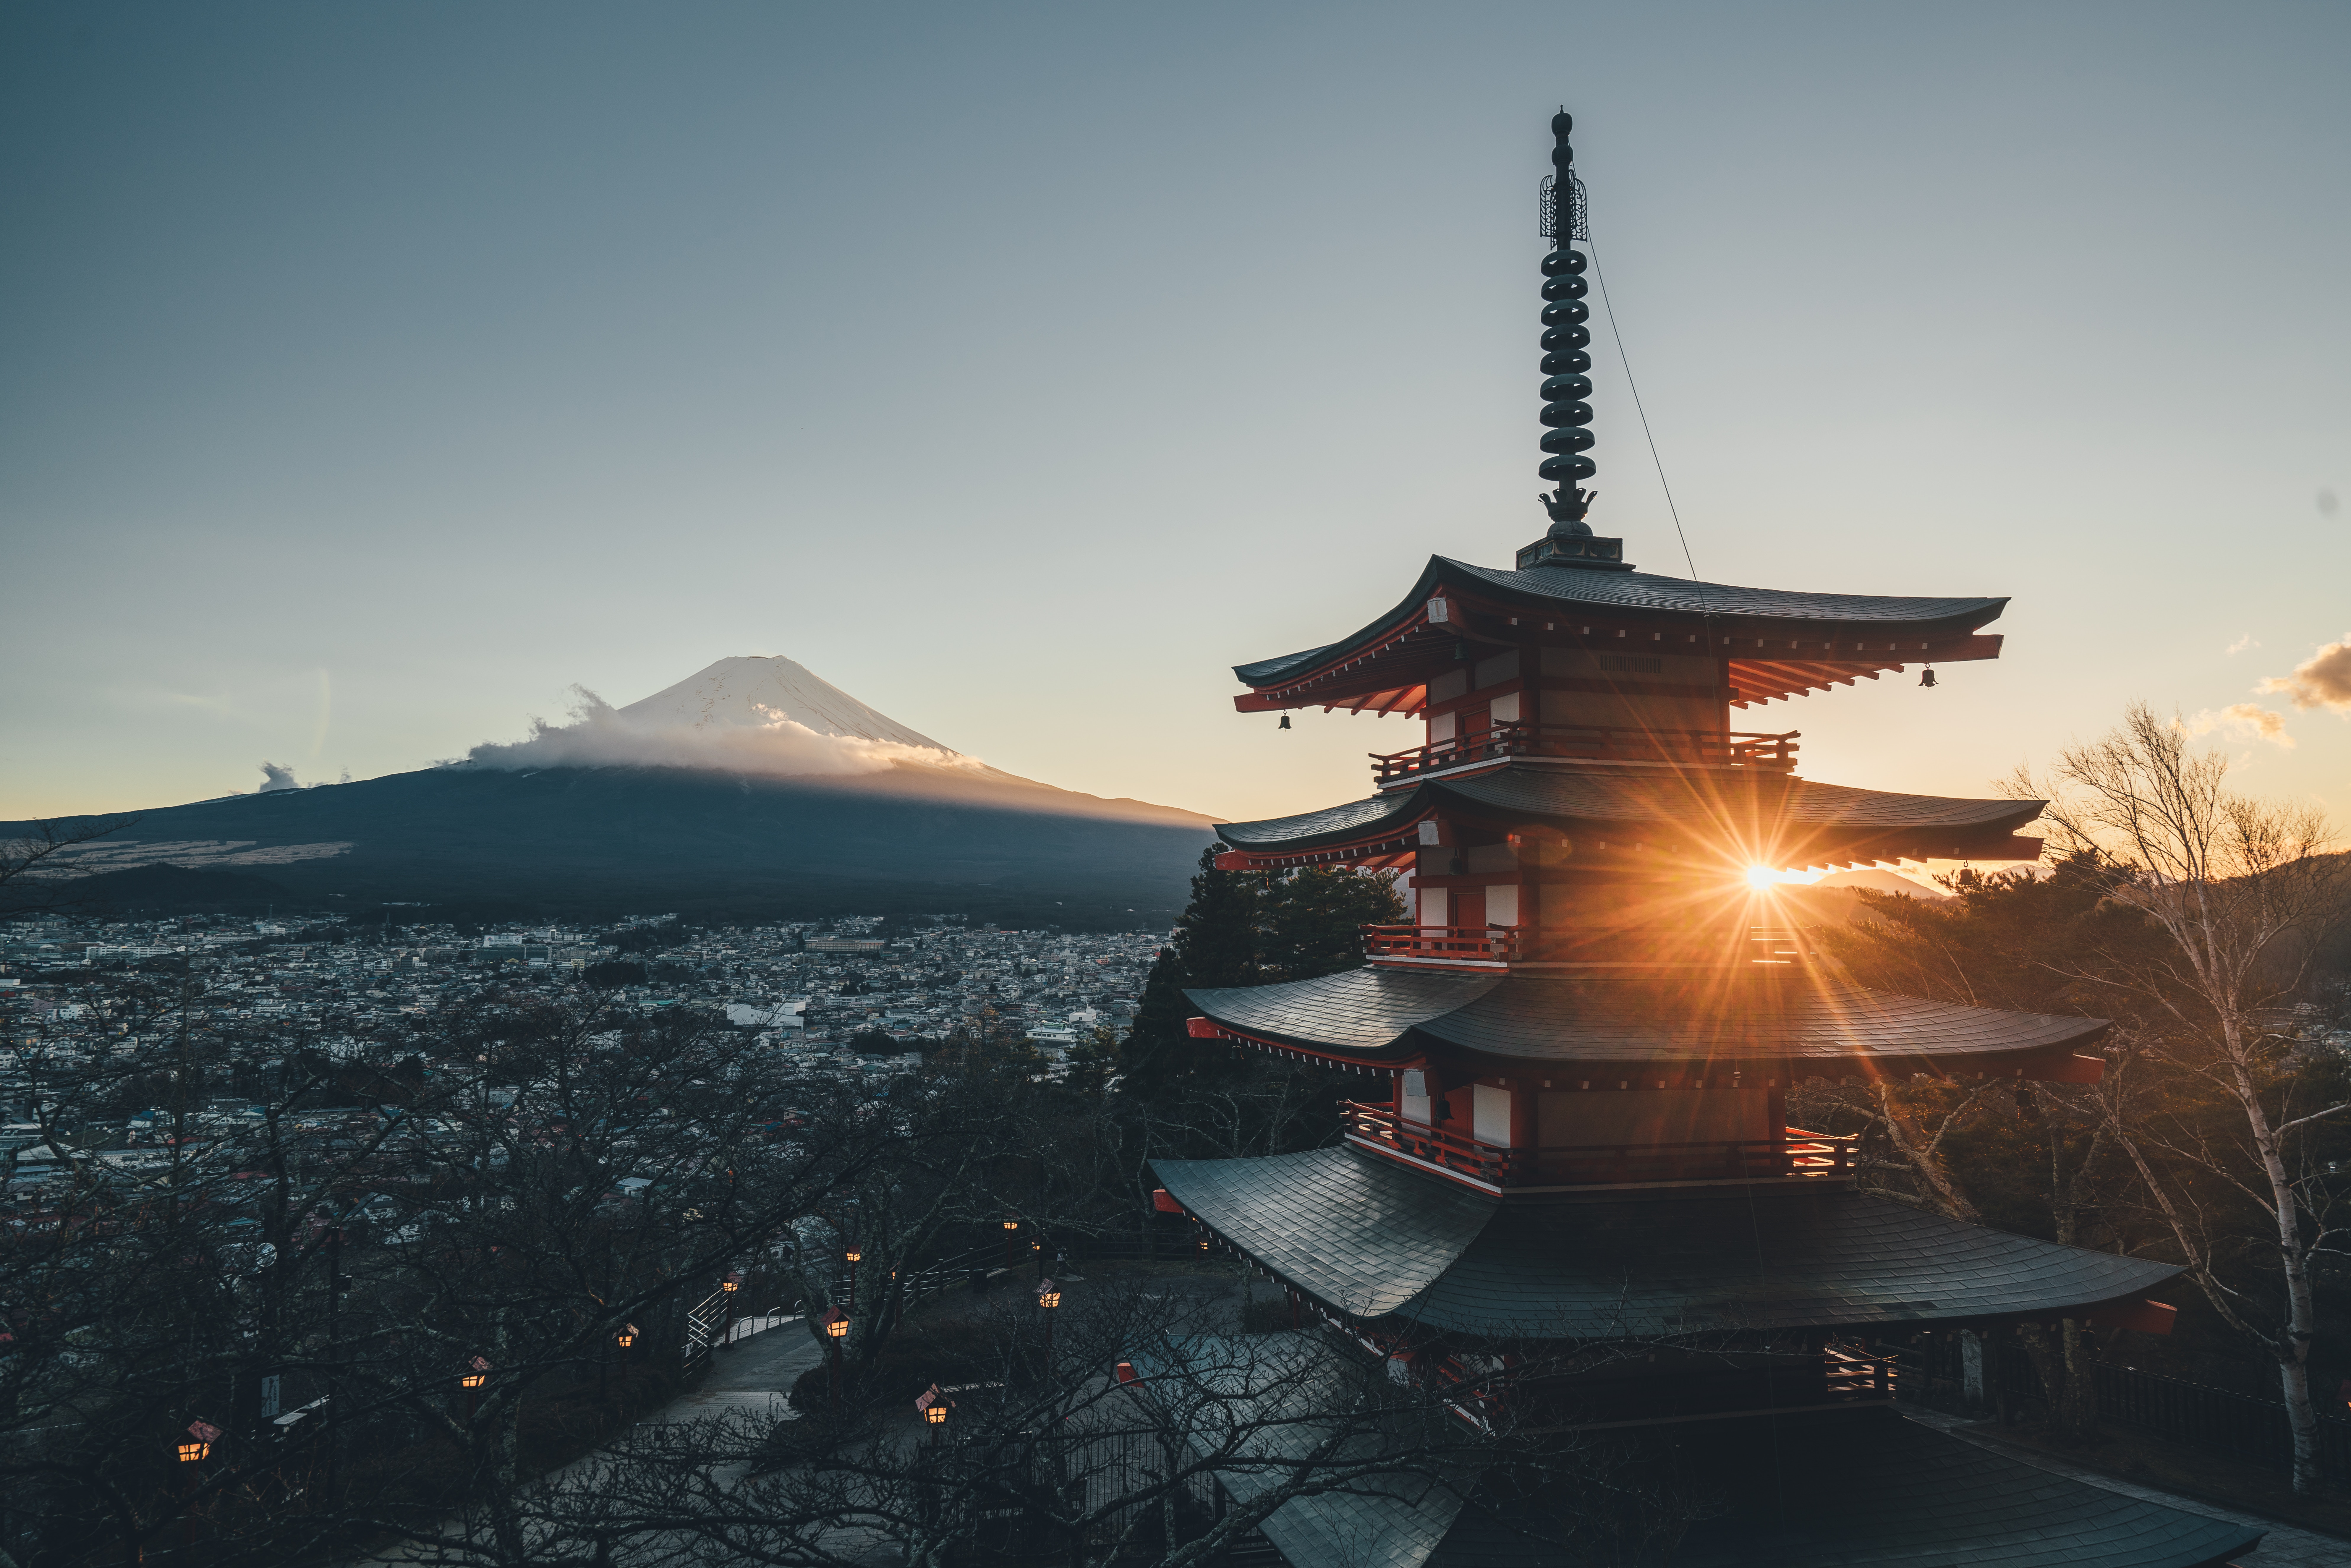
\includegraphics[scale=0.5]{2.png}
    \label{fig:2}
\end{figure}
我们先通过命令行查看虚拟机的IP地址。
\begin{figure}[H]
    \centering
    \includegraphics[scale=0.6]{3.png}
    \label{fig:3}
\end{figure}

然后我们访问这个文件。
\begin{figure}[H]
    \centering
    \includegraphics[scale=0.4]{4.png}
    \label{fig:4}
\end{figure}
可以看到Wireshark捕获到的内容:
\begin{figure}[H]
    \centering
    \includegraphics[scale=0.6]{5.png}
    \label{fig:5}
\end{figure}
我们先来点开第一条消息分析一下。对于第一条消息,为TCP原型。
\begin{figure}[H]
    \centering
    \includegraphics[scale=0.6]{6.png}
    \label{fig:6}
\end{figure}
Frame,指的是物理层的数据帧概况
\begin{figure}[H]
    \centering
    \includegraphics[scale=0.6]{7.png}
    \label{fig:7}
\end{figure}
Ethernet II,第0-13个字节,表示数据层以太网帧头部信息,包含目的地址、源地址和协议类型
\begin{figure}[H]
    \centering
    \includegraphics[scale=0.6]{8.png}
    \label{fig:8}
\end{figure}
Internet Protocol Version 4,第14-33个字节,互联网层IP包头部信息。
\begin{figure}[H]
    \centering
    \includegraphics[scale=0.5]{9.png}
    \label{fig:9}
\end{figure}
Transmission Control Protocol,第34个字节开始,传输层的数据段头部信息。
\begin{figure}[H]
    \centering
    \includegraphics[scale=0.5]{10.png}
    \label{fig:10}
\end{figure}
然后我们观察我们的网页。通过对比可以发现HTTP消息格式为在原有TCP格式的基础上,增加超文本传输协议部分。
\begin{figure}[H]
    \centering
    \includegraphics[scale=0.5]{11.png}
    \label{fig:11}
\end{figure}
然后是三次握手的过程:
\begin{enumerate}
  \item 第一次握手:客户端发送syn包(seq=x)到服务器,并进入SYN\_SEND状态,等待服务器确认
  \item 第二次握手:服务器收到syn包,必须确认客户的SYN(ack=x+1),同时自己也发送一个SYN包(seq=y),即SYN+ACK包,此时服务器进入SYN\_RECV状态
  \item 第三次握手:客户端收到服务器的SYN+ACK包,向服务器发送确认包ACK(ack=y+1),此包发送完毕,客户端和服务器进入ESTABLISHED状态,完成三次握手.
\end{enumerate}

\begin{figure}[H]
    \centering
    \includegraphics[scale=0.4]{12.png}
    \label{fig:12}
\end{figure}
然后使用过滤器进行查找我自己的信息。可以看到,采用的是HTTP/1.1,使用双端口进行连接,防止头阻塞。
\begin{figure}[H]
    \centering
    \includegraphics[scale=0.6]{13.png}
    \label{fig:13}
\end{figure}
可以找到我们所需的信息,和写的html文件是一样的。
\begin{figure}[H]
    \centering
    \includegraphics[scale=0.4]{142.png}
    \label{fig:14}
\end{figure}
接下来是图片。这里是利用GET请求图片文件。
\begin{figure}[H]
    \centering
    \includegraphics[scale=0.4]{15.png}
    \label{fig:15}
\end{figure}
具体信息如下所示:
\begin{figure}[H]
    \centering
    \includegraphics[scale=0.4]{16.png}
    \label{fig:16}
\end{figure}
最后是四次挥手。TCP四次挥手过程:
\begin{enumerate}
  \item 第一次挥手:Client发送一个FIN,用来关闭Client到Server的数据传送,Client进入FIN\_WAIT\_1状态。
  \item 第二次挥手:Server收到FIN后,发送一个ACK给Client,确认序号为收到序号+1(与SYN相同,一个FIN占用一个序号),Server进入CLOSE\_WAIT状态。
  \item 第三次挥手:Server发送一个FIN,用来关闭Server到Client的数据传送,Server进入LAST\_ACK状态。
  \item 第四次挥手:Client收到FIN后,Client进入TIME\_WAIT状态,接着发送一个ACK给Server,确认序号为收到序号+1,Server进入CLOSED状态,完成四次挥手。
\end{enumerate}
\begin{figure}[H]
    \centering
    \includegraphics[scale=0.4]{17.png}
    \label{fig:17}
\end{figure}
\section{总结与一些问题}
我还探究了一些其他内容。比如:TCP包中的win代表接收窗口的大小,即表示这个包的发送方当前还有多少缓存区可以接收数据。Timestamps在tcp选项中包括两个32位的timestamp: TSval(Timestamp value)和TSecr(Timestamp Echo Reply)。如果设置了TS这个选项,发送方发送时,将当前时间填入TSval,接收方回应时,将发送方的TSval填入TSecr。同时发现,当第一次请求页面并请求成功时,页面会返回状态码200表示请求成功,并同时返回页面的html内容;当再次请求且页面没有修改时会返回304表示页面未修改可以直接使用浏览器缓存的内容。因此如果要实际展示,应该先清除缓存,再展示内容。
\end{document}